
\documentclass[paper=a4, fontsize=12pt]{scrartcl} 

\usepackage[left=2.7cm,right=2.7cm,top=2.5cm,bottom=2.5cm]{geometry}
\usepackage[utf8]{inputenc} 
\usepackage{mathpazo} % Palatino font
\usepackage{microtype}
\usepackage[T1]{fontenc}
\usepackage{fourier}
\usepackage[english]{babel}
\usepackage{amsmath,amsfonts,amsthm}
\usepackage{lipsum}
\usepackage{caption}
\usepackage{subcaption}
\usepackage{graphicx}
\usepackage{float}
\usepackage{blindtext} 
\usepackage[hidelinks]{hyperref}
\usepackage{sectsty}
\usepackage{natbib}
\usepackage{caption} 
\usepackage{ragged2e}
\usepackage{tabularx}


\sectionfont{\centering \normalfont\scshape}
\subsectionfont{\centering \normalfont \scshape}
\subsubsectionfont{\normalfont\itshape}

% note divider
\newcommand{\notedivider}{%
	\vspace{4pt}%
	{\hrule height 0.4pt}%
	\vspace{6pt}%
	{\hrule height 0.4pt}
	\vspace{6pt}
}

\captionsetup{font={normal}, 
	labelfont=bf} % sans serif figure and table captions

\usepackage{fancyhdr} % Custom headers and footers
\pagestyle{fancyplain} % Makes all pages in the document conform to the custom headers and footers
\fancyhead[L]{} % No page header - if you want one, create it in the same way as the footers below
\fancyhead[R]{}
\fancyhead[C]{}
\fancyfoot[L]{} % Empty left footer
\fancyfoot[C]{\thepage} % Empty center footer
\fancyfoot[R]{} % Page numbering for right footer
\renewcommand{\headrulewidth}{0pt} % Remove header underlines
\renewcommand{\footrulewidth}{0pt} % Remove footer underlines
\setlength{\headheight}{13.6pt} % Customize the height of the header

%\numberwithin{equation}{section}
%\numberwithin{figure}{section} 
%\numberwithin{table}{section} 
\setlength\parskip{4pt}
\setcounter{secnumdepth}{3}
\setcounter{tocdepth}{3}


\begin{document}
	
	\setcitestyle{authoryear,square,aysep={,},yysep={;}} %bloody hell this took a while but use this for commas between author, year with natbib
	\bibliographystyle{apalike}
	%\renewcommand{\bibfont}{\sffamily\footnotesize}
	
	%----------------------------------------------------------------------------------------
	%	TITLE PAGE
	%----------------------------------------------------------------------------------------
	
	\begin{titlepage} % Suppresses displaying the page number on the title page and the subsequent page counts as page 1
		\vspace*{5em} % star for top of page
		\newcommand{\HRule}{\rule{\linewidth}{0.5mm}} % Defines a new command for horizontal lines, change thickness here
		
		\centering % Centre everything on the page
		
		
		\textsc{\LARGE University of Bristol}\\[1.5cm] % Main heading such as the name of your university/college\textsc{}
		\vspace{-3em}
		\textsc{\Large MSc Bioinformatics}\\[0.5cm] % Major heading such as course name
		\vspace{3em}
		
		%\HRule\\[0.4cm]
		
		{\Large\bfseries Effect of Forest Age on Machine Learning Generalisation of Evapotranspiration Using FLUXNET Data NOTES}\\[0.4cm] % Title of your document
		Fig.~\ref
		\vspace{3em}
		
		%	\HRule\\[1.5cm]
		
		%------------------------------------------------
		%	Author(s)
		%------------------------------------------------
		
		\begin{minipage}{0.4\textwidth}
			\begin{flushleft}
				\large
				\textit{Author}\\
				Archie \textsc{Benn} % Your name
			\end{flushleft}
		\end{minipage}
		~
		\begin{minipage}{0.4\textwidth}
			\begin{flushright}
				\large
				\textit{Supervisor}\\
				Professor Martin \textsc{De Kauwe} % Supervisor's name
			\end{flushright}
		\end{minipage}
		
		\vspace{5em}
		\begin{abstract} 
			{\noindent{\textsc{Abstract} (The abstract has a  maximum of 200 words})}
			\newline
			%\lipsum[1-10][1-20]
			
			\begin{itemize}
				\item Summary of background on ET/ML methods and FLUXNET 
				\item Overall aim of the project 
				\item Proposed approach for the project
			\end{itemize}
			
			\vspace{1em}
			\textit{\textbf{Key words:}} Machine Learning, FLUXNET, Evapotranspiration.\\
			\textit{\textbf{Word count:}} 3000
		\end{abstract}
	\end{titlepage}
	
	\newpage
	\tableofcontents
	\newpage

	
	\newpage
	
	%------------------------------------------------
	% LIT REVIEW
	%------------------------------------------------
	
	\section{Literature Review (3000 words)}
	\subsection{Evapotranspiration and The Water Cycle \\ \textit{(Why does the water cycle matter?)}}
	\subsubsection{Evapotranspiration and Eddy Covariance} 
	\begin{itemize}
		\item Overview of evapotranspiration (ET) (from \citep{wang2012review}):
		\begin{equation}
			ET = Transpiration + E_{Vegetation} + E_{Soil}
		\end{equation}
		\item ET as a crucial component of the energy cycle between terrestrial ecosystems and the atmosphere.
		\item It participates in the water and carbon cycles, reflects the allocation and utilization of the planet’s water resources, and directly affects meteorological phenomena, climate change, and ecosystem functionality through processes such as soil evaporation, plant transpiration, and canopy interception \citep{xue2025review}.
		\item How this plays into the water cycle globally/regionally/in watersheds more generally.
		\item Drivers of ET e.g Leaf Area index (LAi), Vapour pressure deficit (VPD), precipitation, air temperature etc.
		\item Importance and applications of ET predictability
	\end{itemize}
	\notedivider
	\textbf{From \citep{amani2023review}:}
	
	
	
	\newpage
	\subsubsection{Forest age and ET}
	\begin{itemize}
		\item Overview of eddy covariance and briefly how flux tower data collection
		\item How this relates to ET
		\item FLUXNET and how sites are grouped (region and vegetation types)
	\end{itemize}
	\notedivider
	
	\newpage
	\subsection{Changing Forests\\ \textit{(How is climate change affecting forest age?)}} 
	\notedivider
	\subsubsection{Climate Change}
	\begin{itemize}
		\item Overview of climate change and effects on water cycle via carbon dioxide levels/temp. etc.
		\item How these could link to factors such as changing ET
		\item Issues of rapidly changing ET/inability to predict accurately
	\end{itemize}
	\notedivider
	
	\newpage
	\subsection{Evapotranspiration Prediction\\ \textit{(What don't we know and what are the issues?)}}
	\subsubsection{Contemporary ET Prediction Methods}
	\begin{itemize}
		\item Very brief description of non-ML methods for background e.g from \cite{xu2018evaluating}
		\item Disagreement of current satellite and process-based models (between and within)- lack of theory
		\item Lead into ML methods
	\end{itemize}
	\notedivider
	
	\textbf{From \citep{xue2025review}:} 
	\begin{itemize}
		\item Traditional methods, which are computationally simple and data demanding, may fail to accurately capture small-scale ET variations. 
		\item Remote sensing methods provide continuous environmental data for large-scale ET estimation but are constrained by the resolution and quality of remote sensing data. 
		\item Machine learning methods, by extracting features from big data, increase the precision of ET estimation, particularly in data-rich regions. However, the performance of these methods may be limited in data-scarce areas, and model complexity can lead to difficulties in interpretation.
	\end{itemize}
	\notedivider
	\textbf{From \citep{yan2023deep}, an example of an empirical prediction methods' shortcomings:}
	\begin{itemize}
		\item Although the FAO-56 PM equation has been recommended as the standard equation to calculate $ET_0$, it requires complete climatic data which are often not available, limiting its application in data-scarce regions.
		\item In summary, the performance of the standalone HS model cannot be significantly improved by standard local calibrations since these operations can only exert linear changes in the estimations, and thus the proposed approach can further improve the current practice of evaporative capability estimations. (equation \ref{eqn:hs}).
	\end{itemize} 
	
	
	\newpage
	\subsubsection{Machine Learning Models for ET Prediction}
	\begin{itemize}
		\item Brief overview of current ML methods in ET prediction
		\item Performances of different models in the literature 
		\item Look into coupled models (e.g ML-ML coupled like ensembles, or Empirical-ML models such as HS-LSTM from \cite{yan2023deep}).
	\end{itemize}
	\notedivider
	
	\begin{table}[H]
		\centering
		\caption{Advantages and limitations of ML models in the literature.}
		\label{tab:ml_models}
		\begin{tabularx}{\textwidth}{X*{5}{>{\arraybackslash}X}} 
			\hline \hline \\
			\textbf{Method} & \textbf{Advantages} & \textbf{Limitations \& Unresolved} \\
			
			Random Forest \citep{xu2018evaluating} & Outperformed other models (ANN, cubist, SVM, DBN) based on $R^2$, MAPE, RMSE, and relative uncertainties from three-cornered hat. \newline \newline RF  has an ability to handle complex nonlinear relationships between flux and climate and environmental predictors. & Model performs better over areas of dense vegetation compared to barren land. \newline \newline More spatiotemporal continuous land surface variables at fine resolution should be added to potentially enhance predictability.\\
			
			\hline
			\\
			
			HS-LSTM coupled model \citep{yan2023deep} & Shown to outperform the standalone ML and classical $ET_0$ models (RMSE reduced $\sim$20\%). \newline\newline Can be used to estimate future ET$_0$ with only air temperature forecasts which can be easily obtained. & Slight underestimates of extreme $ET_0$ values. \newline\newline Each station required a differently-tuned model, so further studies are required to evaluate potential for a generally valid model and assess whether transfer learning may be applied across different regions. \\
			
			\hline
		\end{tabularx} 
	\end{table}

	\newpage
	\subsection{Project Scope and Machine Learning Applicability\\ \textit{(What is the case for using ML here?)}}
	\subsubsection{Project Scope}
	\begin{itemize}
		\item Address explicit question being asked in project 
		\item "As climate change restructures forest age distributions globally, do ML models trained on historical flux data from forests of one age generalise to forests of different ages?"
		\item Can an ML model trained on a young forest quantitatively predict ET in an older forest without retraining?
		\item Where exactly does model performance break down — is it gradual or is there a threshold age effect?
		\item Which ML architectures are more robust to this — does RF handle it better than LSTM for example?
		\item Which features drive the age-related generalisation failure — is it LAI, VPD response, stomatal conductance?
		\item If a model trained on a mature forest is then applied to a recently burned/disturbed area (which is increasingly common with climate change), how wrong is it?
		\item LAI is arguably the mechanistic link between forest age and ET. Including it raises a really interesting question: does the model generalise better with LAI included or without?
		\item Two experimental designs this opens up:\\
		(1) Model 1: meteorological variables only\\
		(2) Model 2: meteorological variables + LAi\\
		Compare generalisation performance between them — that's a neat additional contribution with minimal extra work
	\end{itemize}
	\notedivider
	
	\newpage
	\subsubsection{Why is ML applicable here?}
	\begin{itemize}
		\item Why is ML important for this specific question?
		\item Include why this is addressable now
		\item Why is there scope to extract more from the FLUXNET data? - high temporal resolution? Multi year? How does this lend itself to ML modelling?
	\end{itemize}
	\notedivider
	
	%------------------------------------------------
	% PROJECT PLAN
	%------------------------------------------------
	
	
	\newpage
	\section{Project Aims and Objectives (500 words)}
	\subsubsection{Aims}
	\begin{itemize}
		\item Overview of how this project will answer the question/area proposed at end of introduction.
	\end{itemize}
	\notedivider
	
	\newpage
	\section{Project Plan (500 words)}
	\subsubsection{Data Acquisition and Selection}
	\begin{itemize}
		\item How the data will be accessed and stored (FLUXNET).
		\item Time period (requires long term sites) and geographical location of data selected for modelling.
		\item Why these were selected and appropriate? (in terms of location/times, not specific structure).
	\end{itemize}
	\notedivider
	
	\newpage
	\notedivider
	\subsubsection{Feature Engineering}
	\begin{itemize}
		\item Selection of data features for use in training and why.
		\item How these were removed or adapted
		\item Why are these features appropriate?
	\end{itemize}
	\notedivider
	
	\newpage
	\subsubsection{ML Model Setup and Training}
	\begin{itemize}
		\item How the data will be accessed and stored (remote sensing and FLUXNET).
		\item Explanation of model(s) selection (type of ML method)
		\item e.g If including LAi vs. not with other parameters kept identical across 2 models.
		\item Overview of model parameters (- might be too much detail?) and how each are trained.
		\item Why are these model choices/parameters appropriate for this task?
		\item Target features: FLUXNET latent heat flux (ET approximation)
		\item Predictor features: Meteorological data (from FLUXNET and others like LAi)
	\end{itemize}
	\notedivider
	
	\textbf{From \citep{xu2018evaluating}:} \textit{``ET was trained and predicted under different land cover types with the following equation:''}
	\begin{equation}
		ET_i = M\left(R_{si},\sum_{i=30}^{i}P_{i},LAI_{i},T_{ai},RH_{i}\right)
	\end{equation}
	
	\textit{``...where $M$ is the training model; $ET_i$ is the target variable; Solar radiation ($R_s$), Precipitation( $P$), Leaf area index ($LAI$), Air temperature ($T_a$), and relative humidity ($RH$) are the explanatory variables; and $P$ is the cumulative precipitation for the 30-day period prior to $i$th day. The subscript $i$ stands for $i$th day.''}
	
	\newpage
	\subsubsection{ML Model Evaluation}
	\begin{itemize}
		\item Testing methods on unseen/held out historical (same as training e.g 5-20 years old) validation sets
		\item Comparison to other predictive models e.g in FLUXCOM
		\item Overall evaluation of model predictability on historical data
	\end{itemize}
	\notedivider
	
	\textbf{From \citep{xu2018evaluating}:} \textit{``The global k-fold testing was adopted to examine the performance of each machine learning method. In this study, 36 sites (65 site years) of flux tower observations were divided into k parts (k = 10 herein). In each training, k 1 parts of data were used as the training data, and the kth part of data was used as the validation data. The cross-validation process was repeated k times (all the data set should be trained and validated), and the results of the evaluation index were then averaged as the assessing results. Although k-fold testing is time consuming for operational application, the data are fully used and the model can lead to more accurate results than the residual testing method.''}
	
	\begin{figure}[H]
		\centering
		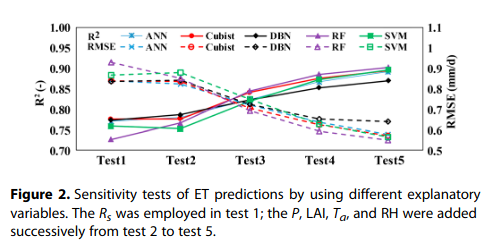
\includegraphics[width=0.75\textwidth]{photos/xu2018.png}
		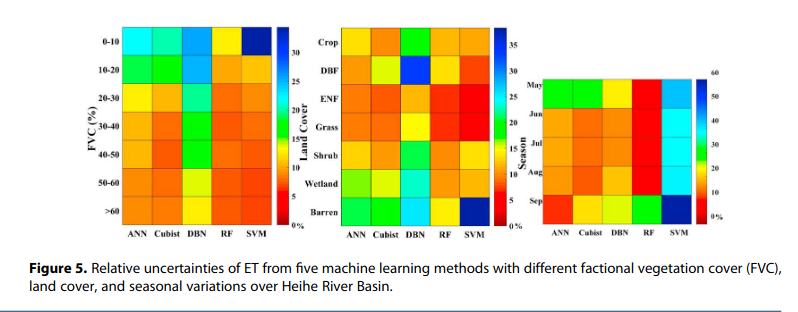
\includegraphics[width=0.75\textwidth]{photos/xu2018_2.png}
		\captionsetup{justification=centering}
		\caption{Examples of some comparisons and testing of model performance in \cite{xu2018evaluating}}
		\label{fig:pldt}
	\end{figure}
	
	
	\newpage
	\notedivider
	\subsubsection{ML Model Predictions}
	\begin{itemize}
		\item Predictions made on unseen and more recent data (e.g last 5 years)
		\item Overall evaluation of model predictability on recent data
	\end{itemize}
	\notedivider
	
	\newpage
	\subsection{Gantt Chart}
	
	\begin{figure}[H]
		\centering
		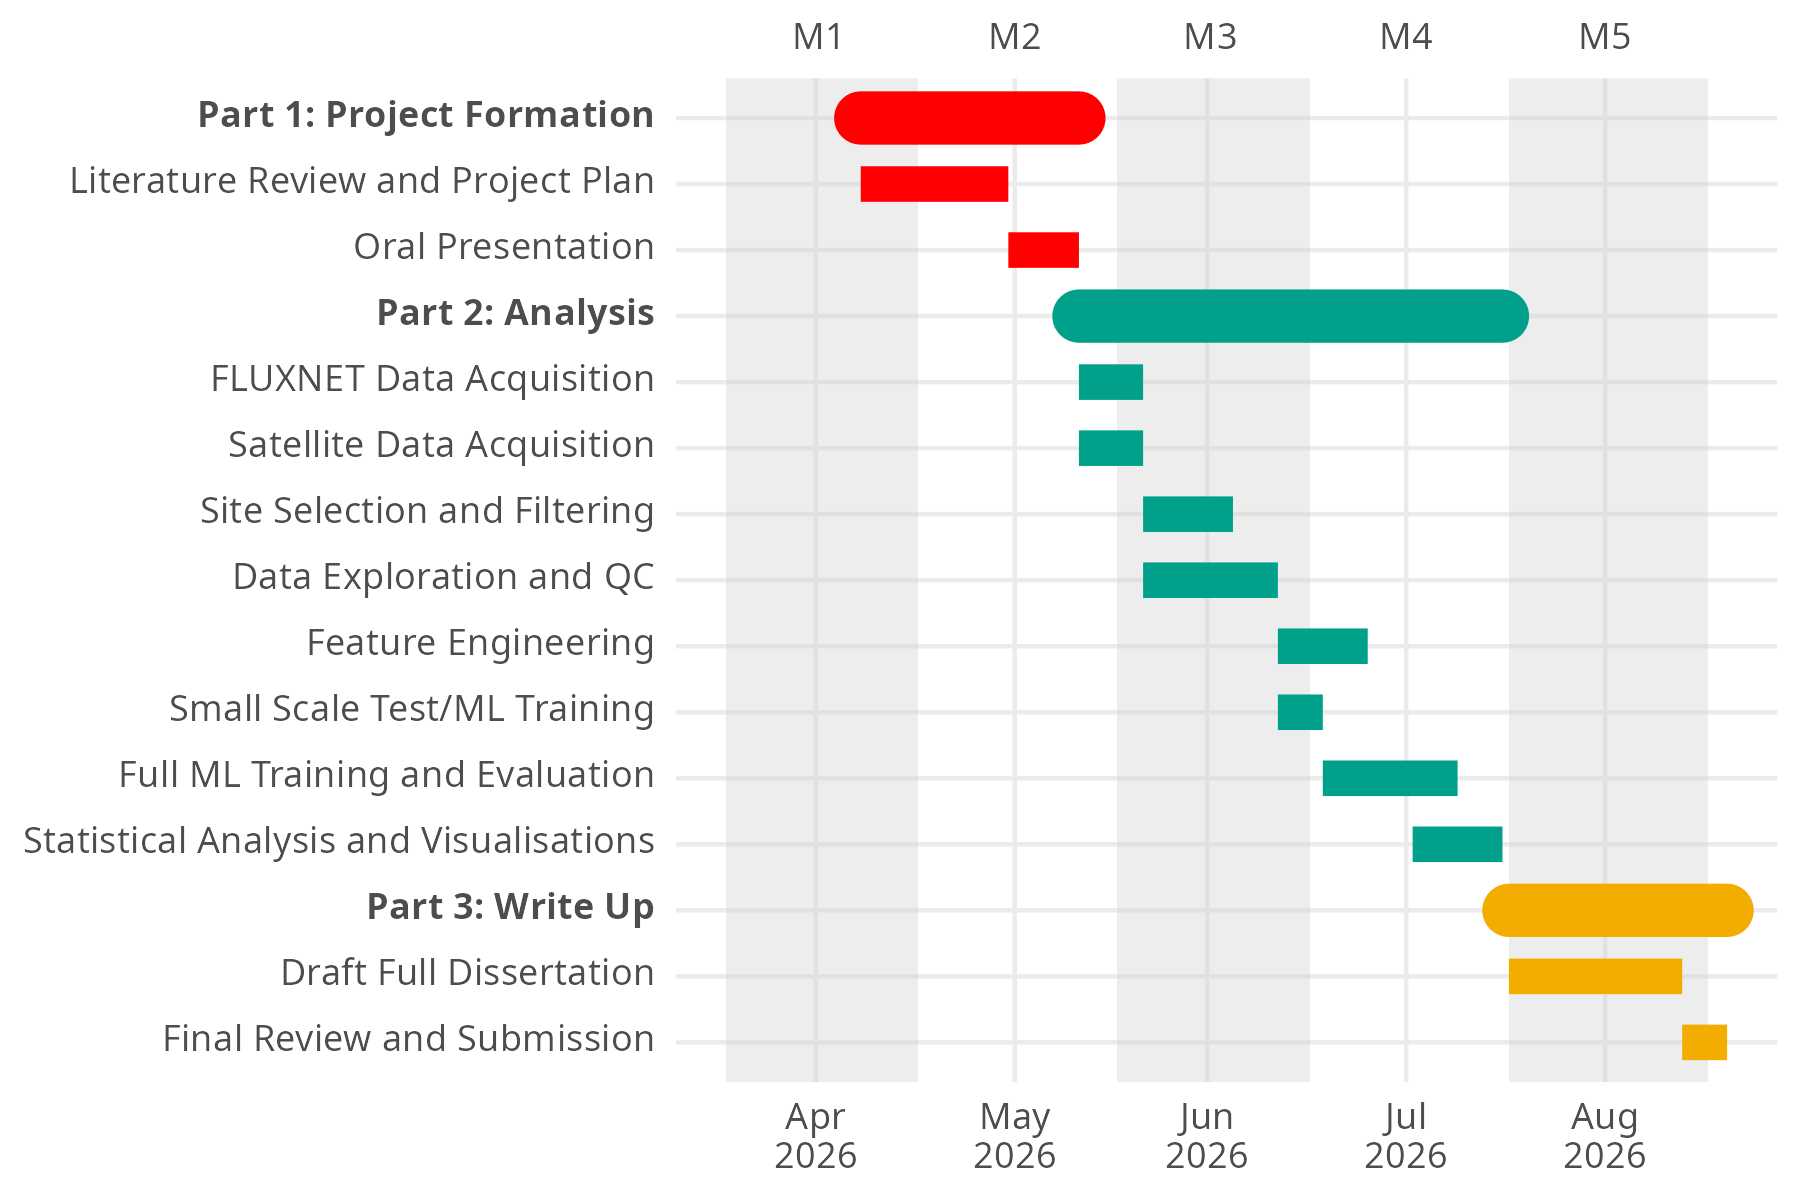
\includegraphics[width=\textwidth]{gantt/gantt1.png}
		\captionsetup{justification=Centering}
		\caption{A proposed Gantt Chart for the duration of this project.}
		\label{fig:gantt}
	\end{figure}
	
	
	
	
	%------------------------------------------------
	% RISK REGISTER
	%------------------------------------------------
	
	\newpage
	\section{Risk Register ($\sim$ 250 words)}
	\begin{itemize}
		\item 4-5 risks at about 50 words each
		\item Data access issues, overfitting, data gaps etc.
	\end{itemize}
	
	\newpage
	\section{Papers}
	\subsection{Evaluating Different Machine Learning Methods for Upscaling Evapotranspiration from Flux Towers to the Regional Scale \citep{xu2018evaluating}
	}
	\subsubsection{Introduction}
	\begin{itemize}
		\item upscale ET from 36 flux tower sites (65 site years) to regional scale
		\item ML methods: artificial neural network, cubist, deep belief network, RF, and support vector networks
		\item essentially took these methods and trained on those 65 years...
		\item then applied to estimate on each grid cell within a watershed between 2012-2016  
		\item deep belief was worst, others had similar performance, and RF had lowest relative uncertainty
		\item ML performed better on densely vegetated conditions than barren/sparse land
		\item "Satellite sensors detecting two-dimensional information of land surface become an effectiv>
		\item 1) predictive equations which link ET observations (flux towers) to vegetation indices 
		\item 2) "geostatistical methods" based on kriging theoretical framework  
		\item 3) using semi-theoretical or running theoretical methods  
		\item 4) using ML methods  
		\item "All of these studies (lists ML methods for ET flux predictions) trained the machine learni>
	\end{itemize}
	
	\subsubsection{Methods}
	\begin{itemize}
		\item went over the 5 ML methods  
		\item study area and data sets
		\item looks at specific river basin in China  
		\item goes over how upstream/midstream/downstream areas in basin are characterised by weather and vegetation like '...mountaineous areas with relatively high precip and mainly covered by grassl>
		\item hydrometeorology observation network was set up within the basin in 2008-2011  
		\item ET observations from eddy covariance (EC) towers (flux towers) was used to test the ML models performance   
	\end{itemize}
	
	\subsubsection{Results}
	\begin{itemize}
		\item Models were sensitive to all the variables in the models, so including all was beneficial.
		\item performance of the 5 models was tested against observed EC data 2012-2016 using R-squared plot  
		\item all 5 rough;y followed 1:1 line, with R-2 values of 0.87-0.89  
		\item RMSE was also calculated alongside MAPE (?)  
		\item so performance evaluated using R-2, RMSE, and MAPE  
		\item as all relatively similar, relative uncertainty was important with 3 cornered hat method  
		\item RF model slightly outperformed the other ML methods based on R2, MAPE, RMSE and relative uncertainties   
		\item therefore RF model was taken forward to predict 2012-2016 over river basin  
	\end{itemize}
	
	\subsubsection*{Limitations and Unresolved}
	\begin{itemize}
		\item Heihe River Basin, the 36 site observations (65 site years; sample number is 65 site year × 365 day/year = 23,725) is not large enough for deep belief network (DBN) model training. Thus, the DBN algorithm underperformed other four algorithms in this study.
		\item larger dataset than the one used here would be better for deep learning models  
		\item ET is also a function of other variables, such as land surface temperature, wind speed, and soil type (or water storage capacity) which were not included here 
		\item However, wind speed increased RMSE here, soil type couldn't be included due to a large desert area in the basin, and cloud contamination meant  LST was not included either
		\item Models didn't match observations perfectly, largely due to: \newline 
		1) ML models simply learn statistical patterns, rather than causal relationships between the included variables ie. can predict well on average but can misrepresent underlying physics. \newline 
		2) truth/observation data isn't exact - EC measurements used here have an uncertainty of about 16\% (wang, 2015). Some mismatch between predictions and observed is expected even in a perfect model as comparing against an imperfect reference. \newline
		3) Higher unertainty in downstream region where there is greater complexity to the land cover types and varying irrigation etc. ML models struggle to capture that spatial complexity which leads to more uncertainty vs. more uniform landscapes.
		\item These 3 compound each other - an imperfect model which doesn't truly understand the physics trained on imperfect data and predicting on a heterogeneous (non-uniform) landscape will inevitable show mismatches.
		\item Models performed much better in vegetation than in barren land, and this is possibly due to the reduced LAi values degrading the models' performances and increasing uncertainties.
	\end{itemize}
	
	
	\subsubsection*{Conclusion/Suggestions}
	\begin{itemize}
		\item ML methods predict better over dense vegetation than sparse region here.
		\item Inclusion of land surface temperature and soil moisture content at fine resolutions could improve the ML performance for ET predictions.  
	\end{itemize}
	
	\subsection{A review of machine learning models and influential factors for estimating evapotranspiration using remote sensing and ground-based data \citep{amani2023review}}
	
	\subsubsection{Introduction}
	\begin{itemize}
		\item Accurate ET estimation is important in understanding ecological and hydrological processes, mitigating droughts, effective water use management/irrigation, and understanding relationship between atmosphere, hydrosphere, and biosphere.
		\item ET is a complex phenomenon influenced by a set of biophysical and environmental factors. Its estimation becomes more complicated in heterogeneous environments, demanding detailed data and accurate model calibration.
		\item ET (top equation) is controlled by factors such as vegetation type, fractional vegetation cover (FVC), phonological cycle, soil type, soil moisture, irrigation and drainage, meteorological conditions, and water management in croplands (i.e. maintaining soil moisture and irrigation management)
		\item ET estimation can be direct or indirect. Eddy covariance is direct (via Latent heat flux), and lysimeter is the most accurate but has issues such as expensive, hard to use, and associated with environmental degredation.
		\item Remote sensing data cannot provide a direct estimation of surface ET; instead, they estimate the retrievable surface parameters associated with ET, such as surface temperature, vegetation indices, and soil moisture.
		\item Point methods can provide ET measurements (e.g flux towers) on a local scale, but the direct measurement of ET on a global scale is impossible, as dense global coverage by such instruments is neither available nor feasible.
	\end{itemize}
	
	\subsubsection{Review Main Points}
	\begin{itemize}
		\item Accurate identification and selection of input data is key to developing an ML model; hence, one should always consider the input data in terms of availability and relevance. Variables affecting ET include climatic factors (maximum and minimum temperature, wind speed, relative humidity, duration, and intensity of solar radiation), soil properties (soil moisture, crop type, agricultural practices, soil texture), and plant properties (plant type, growth stage, leaf shape, total water potential within the leaf) (Allen et al., 1998).
		\item These two datasets act as complementary sources to increase the accuracy of ET estimation.
		\item Liu et al. (2022) investigated the effects of climate change, water fluctuations, and vegetation conditions on ET variation worldwide and identified temperature as the essential determinant of ET in most regions.
		\item The main advantage of ground observation data like FLUXNET is that it is ready to use without any preprocessing steps (Chia et al., 2020).
	\end{itemize}
	
		\begin{figure}[H]
		\centering
		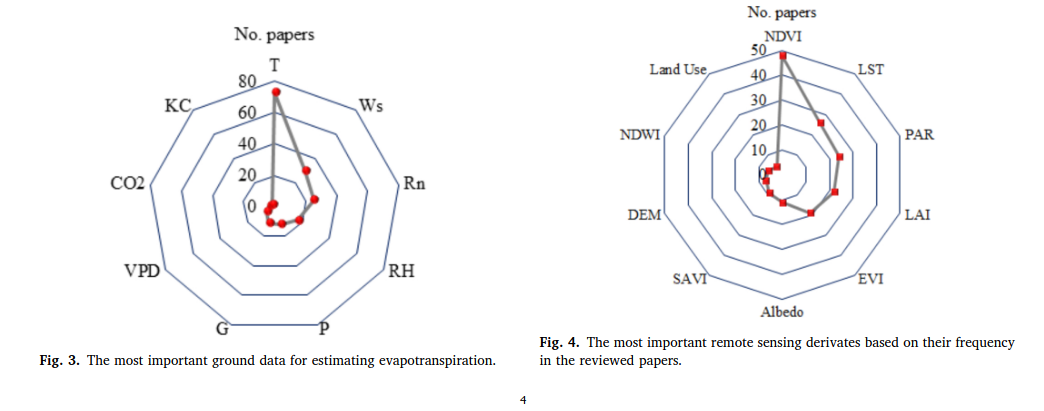
\includegraphics[width=0.95\textwidth]{photos/ground_rs.png}
		\captionsetup{justification=centering}
		\caption{Main variables for ground vs RS ET prediction in this review.}
		\label{fig:plddt}
	\end{figure}
	
	
	\subsubsection{Limitations and Unresolved}
	\begin{itemize}
		\item However, the use of tower/ground based data also has disadvantages; for example, meteorological station measurements only show the conditions of the tower and its proximity (Baldocchi, 2008; Yang et al., 2006), and setting up these is costly, leading to heterogenous distribution of these towers.
		\item In addition, the flux towers are not spatially well distributed, and this heterogeneous distribution leads to significant uncertainties in ET estimation at both regional and global scales (Li et al., 2018).
		\item ML models may struggle with extrapolation, meaning that they may not be able to generalize well beyond the data they were trained on.
		\item ML models may perform comparably or even better than complex physical methods, particularly for the large scale studies, but they do not have the interpretability that physical models do.
		\item accuracy of ML models depends on the quality of satellite and terrestrial data and the representativeness of the samples. There are sevHowever, the use of sucheral uncertainties associated with RS data. Some of these uncertainties include sensor noise, cloud cover, atmospheric interferences, shadows, limitations in spatiotemporal resolution, and satellite viewing angle. 
		\item Satellites with a higher temporal resolution usually have a lower spatial resolution, combining different sensors is necessary to obtain higher frequencies and better spatial resolution.
		\item Geographically, most studies have been conducted in China, the United States, and European countries because of the presence of FLUXNET towers and reliable data for model validation in those areas. Nonetheless, ET estimation in arid and semi-arid regions such as Africa, South Asia, the Middle East, Australia, and the Arctic, is very important, and climate problems and water crises are evident in these areas
	\end{itemize}
	
	
	\subsubsection{Conclusion/Suggestions}
	\begin{itemize}
		\item  1) Advances in RS technology have facilitated the continuous monitoring of biophysical variables affecting ET estimation.\newline
		2) Physics-based models can maintain energy balance but require experimental estimation of some parameters such as surface resistance and determining hot and cold pixels which is challenging for large scale studies or a global scale. \newline
		3) ML models, on the other hand, have reduced uncertainties and yielded more accurate predictions. As can be seen in Fig. 6, the trend of using ML models has been increasing over recent years; the number of papers published has increased sharply in 2020 and 2021, confirming the importance and efficiency of these methods.
		\item The success of ML methods in estimating ET relies heavily on the choice of predictors. For example, the predominant role of vegetation change in controlling global ET changes has been widely reported over the past few decades, while other factors such as CO2 concentration, precipitation, and downward radiation continue to play essential roles in ET estimation.
		\item SVM and ANNs are considerably affected by redundant variables, while RF models show moderate degradation in performance.
		\item Increasing the study area and influential factors, the ML models might be time-consuming mainly when parameter tuning is considered, and especially with input data coming from high-resolution satellite imagery.
		\item It should be noted that single ML models may perform comparably or even better than combined models or separate physical models, depending on the input data, model type, extreme values, etc. However, to get the best results in situations where we deal with a complex phenomenon, it is better to use ensemble models that yield more stable results.
		\item Future studies should examine the limitations and accuracy of ET estimation using deep learning models and RS data both for the local and large scale studies.
		\item The development of FLUXNET towers in these areas is reasonably necessary, because ML models require large amounts of quality data to train effectively. If the data is biased or incomplete, then the model may not be able to generate accurate predictions. Hence, other ground-based ET observations and FLUXNET towers in arid and semi-arid regions can reduce uncertainty of ET estimation.
	\end{itemize}
	
	\newpage
	\subsection{A Review of Evapotranspiration Estimation Models: Advances and Future Development \citep{xue2025review}}
	\subsubsection{Introduction}
		
	\begin{itemize}
		\item Traditional methods, which are computationally simple and data demanding, may fail to accurately capture small-scale ET variations. 
		\item Remote sensing methods provide continuous environmental data for large-scale ET estimation but are constrained by the resolution and quality of remote sensing data. 
		\item Machine learning methods, by extracting features from big data, increase the precision of ET estimation, particularly in data-rich regions. However, the performance of these methods may be limited in data-scarce areas, and model complexity can lead to difficulties in interpretation.
		\item The empirical methods primarily rely on the relationships among meteorological parameters. While these methods are simple in computation but lack a reliable physical basis and are sensitive to changes in meteorological conditions and surface characteristics. In contrast, machine learning model are data-driven, leveraging both linear and non-linear relationships to establish a mapping between inputs (such as meteorological and soil data) and outputs (ET rates).
	\end{itemize}
	
	\subsubsection{Review Main Points}
	\begin{itemize}
		\item During the nascent phase of ET research, many observational techniques, including the eddy covariance method, bowen ratio method, and lysimeter, were applied at the plot scale (Bowen 1926). These methods are of great significance for the establishment, validation, evaluation of ET models and the training of machine learning models.
		\item ML models are distinguished from conventional approaches by their innate capacity to autonomously distill features from datasets and iteratively refine model parameters, all in the pursuit of minimizing predictive discrepancies (Liu et al. 2024)
		\item ML is used to delineate the intricate interplay between ET and a variety of meteorological and soil data by extracting and assimilating abstractive features from the input dataset. This process cultivates a profound comprehension of the distributional characteristics of the data, encompassing the frequency and probabilistic spread of the data across their spectrum, which in turn empowers the constructed model to more precisely capture and forecast the fluctuating dynamics of ET (Elbeltagi et al. 2023; Hailegnaw et al. 2024).
		\item ML models can be augmented by their synergy with traditional ET estimation techniques that are underpinned by physical mechanisms, culminating in the realization of more holistic and precise estimation outcomes (Feng et al. 2024; Sun et al. 2022b).
		\item Previous studies have utilized flux station data to construct ET estimation models on the basis of ML methods such as random forests, extreme gradient boosting, support vector regression, and artificial neural networks and have conducted comparative studies.
		\item The Hargreaves-Samani long short term memory (HS-LSTM) model, which was proposed by Yan et al. (2023) for estimating daily ET0 and actual ET, was compared with standalone HS, LSTM, adaptive neuro fuzzy inference system (ANFIS), and genetic programming (GP) models, and the HS-ML model was found to outperform the standalone HS and ML methods, with LSTM showing the best performance among the ML algorithms.
	\end{itemize}

	
	
	\subsubsection{Limitations and Unresolved}
	\begin{itemize}
		\item ML methods can provide the best possible constraints for ET on the basis of available data, but the internal complexity of these models makes diagnosing the causes and consequences of uncertainty difficult.
		\item In practical applications, it is necessary to strike a balance between deep learning and traditional methods and to choose the most appropriate solution on the basis of specific circumstances \citep{amani2023review}.
		\item Owing to the complexity of the land surface, differences in model structure, and uncertainty of input data, there are still many challenges in accurately estimating ET.
	\end{itemize}
	
	
	\subsubsection{Conclusion/Suggestions}
	\begin{itemize}
		\item Wang et al. (2022b) reported that DL models could be used with a select array of key types of observational data to effectively simulate actual ET. The study indicated that while enriching the number of in situ observational data types may enhance a model’s generalization capability, it does not significantly enhance simulation precision; thus, the selection of suitable data types is more important than indiscriminately expanding the diversity of the data
		\item Data format transformation optimizes feature extraction, captures spatial correlations within the data, and helps CNNs understand the influences of atmospheric environments in detail. When trained with historical data, CNNs learn the complex relationships between meteorological characteristics and ET, which enables the accurate prediction of future ET (Qin et al. 2022; Yan et al. 2023).
		\item RNNs and LSTM models have distinct advantages in processing time series data. These models capture long-term dependencies within time series data to effectively predict the dynamic changes in ET.
		\item To address these challenges, users should consider the adaptability of the model, the availability of data, the precision requirements for the estimation, and the complexity of technical operations when selecting an ET estimation method. Specifically, users should prioritize models that can adapt to specific climatic and topographic conditions, match data requirements with availability, and provide accurate estimation results after parameterization and calibration and whose technical demands are commensurate with user capabilities.
		\item Following 4 points are made for suggestions:\\
		(1) Expansion of datasets: Increasing the resolution of remote sensing technology and establishing dynamic databases that include detailed information on soil classification, vegetation canopies, and surface reflectance to accommodate different geographical regions and seasonal variations. \\
		(2) Utilization of high-resolution remote sensing data: Employing satellite and drone technology to acquire key parameters such as surface temperature, vegetation indices, and soil moisture, thereby enhancing the data foundation for ET estimation.\\ 
		(3) Development of ML techniques: In particular, DL architectures, such as CNNs and RNNs, are calibrated on the basis of large-scale datasets to improve the accuracy and efficiency of ET estimation.\\
		(4) Refinement of meteorological and hydrological models: Integrating atmospheric and soil hydrological models and considering factors such as terrain, soil, and vegetation to simulate the ET process more accurately.
	\end{itemize}
	
	\newpage
	\subsection{Deep learning for daily potential evapotranspiration using a HS-LSTM approach \citep{yan2023deep}}
		\subsubsection{Abstract/Introduction}
	\begin{itemize}
		\item The present study proposed a novel deep learning (DL) approach for daily $ET_0$ estimations with limited daily climate data: HS- LSTM. This approach was constructed based on a classic ET0 model and a long short-term memory neural network (LSTM).
		\item Hargreaves-Samani (HS) model was employed as the classic model, and the predictors were restricted to the daily maximum and minimum air temperature data.
		\item main objectives of this study were:\\
		 1) to develop temperature-based LSTM based models for estimating daily ET0 using air temperature data;\\ 
		 2) to propose a HS-ML technique for estimating daily ET0; and\\
		 3) to evaluate and compare the estimation capabilities of the standalone HS model, the standalone LSTM approach, and the newly proposed HS-ML approach (HS-LSTM).
	\end{itemize}
	
	\subsubsection{Methods}
	\begin{itemize}
		\item This study was conducted in Songliao Basin, Northeast China.
		\item The historical daily meteorological data ranges from January 1st, 1984 to December 31st, 2019.
		\item The FAO-56 Penman-Monteith (PM) equation (for ground truth), which is the standard formulation to calculate $ET_0$, was employed to compute the historical daily $ET_0$ (ground truths) at the meteorological stations to train, validate, and test the models
		\item The FAO-56 PM equation can be expressed as (Allen et al., 1998):\\
		\begin{equation}
			ET_0 = \frac{0.408\Delta(R_n - G) + \gamma[900/(T + 273)]U_2(e_s - e_a)}{\Delta + \gamma(1 + 0.34U_2)}
		\end{equation}
		where $ET_0$ is the potential evapotranspiration (mm day 1); $\Delta$ is the slope  of vapour pressure curve at a given air temperature (kPa ◦C 1); $R_n$ is the  net radiation at the crop surface (MJ m 2 day 1); $G$ is the soil heat flux  density (MJ m 2 day 1); $\gamma$ is the psychrometric constant (kPa ◦C 1); $T$ is the mean daily air temperature at 2 m height (◦C); $U_2$ is the wind speed at the 2 m height (m/ s); $e_s$ is the saturation vapour pressure (kPa); $e_a$ is the actual vapour pressure (kPa).
		\item Although the FAO-56 PM equation has been recommended as the standard equation to calculate $ET_0$, it requires complete climatic data which are often not available, limiting its application in data-scarce regions
		\item The HS model for $ET_0$ has many forms, but the version used here can be shown as:\\
		\begin{equation}
			ET_0 = 0.0135(T + 17.78)R_s\left(\frac{238.8}{595.5 - 0.55T}\right)
			\label{eqn:hs}
		\end{equation}
		where $T$ is the mean temperature (C) and $R_s$ is the incident solar radiation (MJ m 2 day 1).
		\item In the first phase, standalone ML models were established for ET0 estimations.
		\item In the next phase, HS-ML models were developed.
		\item LSTM is an advanced version of recurrent neural network (RNN) which deals with sequential time series data.
		\item HS-LTSM model (best performing) setup:\\
		(1) Three variables (including $T_{max}$, $T_{min}$, and HS $ET_0$) were used as input variables, and the length of input time step was set as 14 (two weeks). \\
		(2) Two LSTM layers were than used, followed by two dense layers. \\
		(3) ReLu activation function was employed. \\
		(4) The mean squared error (MSE) between the ground truths and estimated data was used as a function. The network was trained to minimize MSE using the Adam optimization algorithm with an initial learning rate of 0.0001.\\
		(5) Batch size set to 64 and models trained for 300 epochs. \\
		(6) To eliminate errors due to measurement units, all data were normalized to fall between 0 and 1. The equation for normalization can be represented as:\\
		\begin{equation}
			X_n = \frac{X - X_{min}}{X_{max} - X_{min}}
			\label{eqn:normal}
		\end{equation} 
		(7) The hyperparameters for the ML models were primarily determined by comparing the evaluation statistics for the validation datasets.
	\end{itemize}
	
	\subsubsection{Results}
	\begin{itemize}
		\item In the present study, the HS model tended to overestimate the $ET_0$ at 6 of the 16 stations, whereas it underestimated the remaining 10 stations. This issue of overestimation or underestimation may be partially resolved by local calibration, i.e., tuning the model coefficient for $R_s$ to improve the model accuracy.
		\item However, the present study found that there was a good match between the ground truths and HS estimations for low $ET_0$ values while there was a poorer match at some stations for high $ET_0$ values.
		\item The proposed HS-LSTM approach also outperformed the other ML algorithms.
		Interestingly, the current study found that the performance results of the standalone traditional ML algorithms were almost equivalent, and they were not found to significantly improve the performance compared to the HS model (Fig. 8). (\textbf{as in \cite{xu2018evaluating}}).
		\item This observation was inconsistent with  most of the previous ML studies, which concluded that ML models outperformed traditional $ET_0$ formulas
	\end{itemize}
	
	\subsubsection*{Limitations and Unresolved}
	\begin{itemize}
		\item In summary, the performance of the standalone HS model cannot be significantly improved by standard local calibrations since these operations can only exert linear changes in the estimations, and thus the proposed approach can further improve the current practice of evaporative capability estimations. (\textbf{limitation of the empirical HS calculation} (equation \ref{eqn:hs}))
		\item leads to deployment/argument for HS-ML model (ML techniques have been well known to be capable of solving nonlinear problems, and this merit may remedy the limitation of the HS model)
	\end{itemize}
	
	
	\subsubsection*{Conclusion/Suggestions}
	\begin{itemize}
		\item  This study proposed a novel ML approach, HS-LSTM, for $ET_0$ estimates that is superior to the classic formulation. In this work, the HS model was employed as a representative traditional ET0 model. As a classical formula for estimating daily $ET_0$, the HS model has been widely used worldwide because of its acceptable accuracy and low requirements for meteorological data (Allen et al., 1998). Recently, Kaya et al. (2021) showed that the HS estimations were more accurate than the estimations provided by the other tested empirical equations (i.e., the Ritchie and Turc equations).
		\item Developing new techniques that rely on a reduced number of variables, which are available from public weather forecast services, is of great importance
		\item Therefore, it is quite common that coupled models exhibit better performance over the standalone models. However, most of the existing studies only coupled different ML algorithms, without utilizing the advantages of classic $ET_0$ equations.
		\item \textbf{Best of both worlds?} On the one hand, the existing empirical or semi-empirical $ET_0$ models were mostly derived using traditional regression techniques, and ML algorithms can compensate for the relatively weaker generalization capability of the traditional regression techniques. On the other hand, the classical ET0 formulation has been widely tested worldwide, and coupling with these formulations was equivalent to providing an additional dataset for the standalone ML algorithms.
	\end{itemize}
	
	\newpage
	\subsection{Machine learning-based investigation of forest evapotranspiration, net ecosystem productivity, water use efficiency and their climate controls at meteorological station level \citep{shi2024machine}}
	
	\subsubsection{Abstract/Introduction}
	\begin{itemize}
		\item In the context of global climate change, assessing changes in the evapotranspiration (ET), net ecosystem productivity (NEP) and ecosystem water use efficiency (EWUE) (Sun et al., 2011; Tian et al., 2016) of global forest ecosystems is important for global carbon neutrality policies and climate adaptation policies.
		\item However, understanding of the global forest carbon and water cycle processes and their  responses to climate change remains complex and uncertain.
		\item Generally, Forest ET represents water consumption from soil evaporation and canopy transpiration and is influenced by environmental factors such as vapour pressure deficit (VPD), soil moisture, solar radiation, air temperature, and wind speed (Yang et al., 2023).
		\item High VPD and strong solar radiation increase ET, while adequate soil moisture and suitable temperatures are necessary to maintain it.
		\item Looks at tree species and how this can affect transpiration etc.
		\item These differences in stomatal strategies reflect each species’ adaptability to environmental conditions and their impact on ecosystem carbon dynamics.
		\item For example, many previous studies did not consider or only used simple representations of the effect of forest age when estimating NEE or NEP. Studies using flux observations (Besnard et al., 2018) have shown that, in addition to climate and soil properties, \textbf{forest age} is powerful in explaining spatial and temporal variations in NEP, and that reliable maps of forest age distributions are important in accurately predicting NEP both spatially and temporally.
		\item \textbf{How to disentangle effects of ET from climate change vs. effects coming from age of forests?}
		\item Random Forest (RF) has been widely utilized in constructing various carbon flux datasets (Jung et al., 2020; Tramontana et al., 2016; Zeng et al., 2020) by upscaling flux observations from the site to the regional scale.
	\end{itemize}
	
	\subsubsection{Methods}
	\begin{itemize}
		\item Consequently, we employ the RF algorithm to estimate daily-scale ET and NEE data from forest meteorological stations worldwide.
		\item This allows us to investigate changes in ET, NEP, and EWUE, as well as their relationships with climate dynamics across various forest ages. The findings of this study provide a meteorological station-level understanding of carbon and water flux dynamics and their response to climate change.
		\item While parameter optimization can enhance accuracy in cross-validation of flux station data, its effectiveness may not necessarily translate when applied to meteorological stations. 
		\item Random Forest (RF), being an ensemble learning method, inherently possesses the ability to largely avoid overfitting. Given this characteristic, we opted to use the default parameters provided in Python’s ’scikit-learn’ library for all parameters except ’n\_estimators’
		\item When calculating NEP, ET, and EWUE on an annual scale (predictions), we filtered out values for years with fewer than 270 days of site records. This ensured a robust dataset for our analysis.
		\item \textbf{Ask Martin about this:} Further, considering the spatio-temporal and nonlinear nature of the Earth system, we employed \textbf{CCM}, a nonlinear state-space causal inference method (Sugihara et al., 2012), to evaluate the effects that Pearson’s correlation methods cannot detect. CCM reconstructs a nonlinear state-space according to Takens’ theorem to reveal causal relationships. Specifically, if we can predict variable X from the reconstruction space of variable Y, then we consider X to have a causal effect on Y, with the causal magnitude measured by the correlation between predicted X and actual X. CCM methods and their derivatives are now widely used in ecology and climate science (Gao et al., 2023; Sugihara et al., 2012). In our study, our X represents climate factors, while Y represents NEP, ET, or EWUE. The specific implementation of CCM relies on the Python package ‘pyEDM’. We used the ‘EmbedDimension’ function to determine the value of the important parameter ‘E’ in the CCM function, while providing larger values for ‘sample’ and ‘libsize’ to ensure convergence and improve the accuracy of results as much as possible.
	\end{itemize}
	
		\begin{figure}[H]
		\centering
		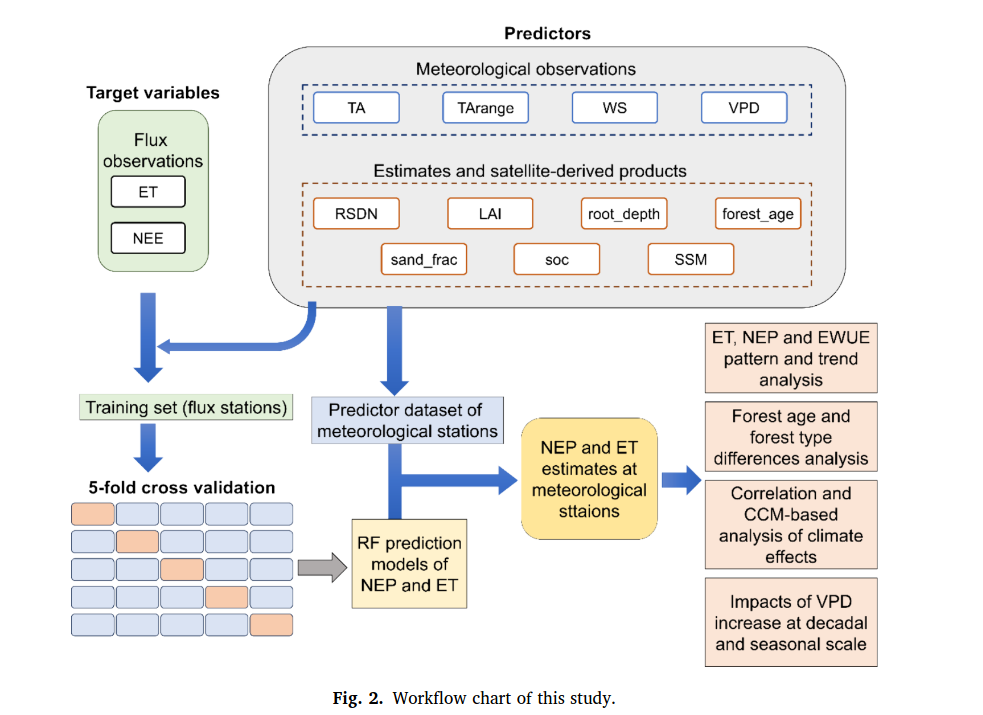
\includegraphics[width=0.95\textwidth]{photos/shi_2024.png}
		\captionsetup{justification=centering}
		\caption{RF model setup for \cite{shi2024machine}.}
		\label{fig:pld}
	\end{figure}
	
	\subsubsection{Results}
	\begin{itemize}
		\item We evaluated model accuracy by 5-fold random cross-validation. The daily-scale ET model had an R-squared of 0.80 and mean absolute error (MAE) of 0.38 mm/d.
		\item In the ranking of feature importance (IMP) of the two models, RSDN, TA, and LAI all ranked relatively high.
		\item Annual scale ET is significantly positively correlated with several variables (e.g. TA, VPD, RSDN). ET and Arid Index (long-term precipitation divided by potential evaporation (Programme, 1997)) showed negative correlations since a lower Aridity Index value represents a higher degree of aridity. It can be explained that the energy limitations in the high Aridity Index region (the more humid regions) correspond to a low ET
		\item This suggests that as VPD rises, the ET of the forests may increase, but changes in NEP and EWUE may not be significant. This suggests that the effect of increased atmospheric moisture demand on ET in forests is significant, but not on NEP and EWUE.
	\end{itemize}
	
	\subsubsection*{Limitations and Unresolved}
	\begin{itemize}
		\item For both process-based modelling and machine learning, the coarse resolution of the forcing data may also cause considerable uncertainties in ET and NEP estimation and in investigating their relations to climate dynamics. 
		\item This may lead to difficulties in dealing with surface heterogeneity when the model is applied. For example, the resolution of climate reanalysis data commonly used in NEE and ET estimation is usually at ~ 10 km scale (Tramontana et al., 2016), which may make it difficult to accurately represent local meteorological conditions (Fig. 1) and environmental controls with high spatial heterogeneity.
		\item Water-related effects may be more important than temperature-related effects at small scales because spatial heterogeneity in precipitation, soil moisture, water vapor, etc., may be higher than temperature, and coarse-scale data and large-scale analyses may offset heterogeneity and underestimate the impact of actual water-related factors (Jung et al., 2017)
		\item It is partially because machine learning tends to underestimate the impact of extreme values (underestimating extremely high values and overestimating extremely low values), thus representation of the response to the impact of extreme events can be inadequate.
	\end{itemize}
	
	
	\subsubsection*{Conclusion/Suggestions}
	\begin{itemize}
		\item This study utilized in-situ meteorological data and machine learning at weather station scales to reassess the variations in global forest carbon and water fluxes and their responses to hydroclimatic changes.
		\item Incorporating more site-specific observations, such as plant traits, could enhance understanding of climate-plant-ecosystem relationships.
		\item Utilizing site-scale data can potentially mitigate the negative impacts of coarse-resolution data and their associated uncertainties. Meteorological stations offer a wider and denser distribution in global forests compared to flux station networks. 
		\item By integrating meteorological station-scale observations, soil moisture data, remote  sensing data, and forest age information, machine learning approaches show promise in estimating ET and NEE at forest meteorological stations. This approach is particularly valuable for reducing errors caused by scale mismatch.
		\item This knowledge is crucial for forest management strategies aimed at achieving carbon neutrality and enhancing climate adaptation. By offering insights at this scale, our research contributes valuable information to support more targeted and effective forest management practices in the face of ongoing climate challenges.
		\item future research could explore the use of advanced hyperparameter optimization tools such as Optuna and Hyperopt. These tools hold the potential to further improve prediction accuracy.
		\item We suggest that future research should focus more on the impact mechanisms of hydroclimatic dynamics on carbon and water fluxes and ecosystem functions at the weather station scale, thereby gaining a deeper understanding of the specific impacts of scale effects in attribution
	\end{itemize}
	
	
	
	\subsection{Evapotranspiration on a greening Earth \citep{yang2023evapotranspiration}}
	\subsubsection{Introduction and abstract}
	\begin{itemize}
		\item Evapotranspiration (ET) — the distribution and partitioning of which is strongly mediated by vegetation
		\item Evapotranspiration (ET) describes the phase transition of water from liquid to gas at the surface, and the subsequent transfer to the atmosphere.
		\item However, there are large uncertainties in the magnitude and spatiotemporal patterns of ET estimates16–18, linked to the inability to observe ET directly from satellite sensors, limited coverage by in situ ET observations and difficulty in parameterizing the complex and intertwined physical and biological processes governing ET at different scales1,19
	\end{itemize}
	
	\subsubsection{Methods}
	\begin{itemize}
		\item  
	\end{itemize}
	
	\subsubsection{Results}
	\begin{itemize}
		\item 
	\end{itemize}
	
	\subsubsection*{Limitations and Unresolved}
	\begin{itemize}
		\item
	\end{itemize}
	
	\newpage \cite{liyew2025review} lists a study with NO age included - just NDVI and LAI. good argument for use of stand age as not used at all. (section 3)
	
	
	% REFERENCES
	\newpage
	\bibliography{references.bib}
	
	
\end{document}
